%
% TURTLE
%
% Documentazione
%

\documentclass[12pt, a4paper]{report}

\usepackage[italian]{babel}
\usepackage[utf8x]{inputenc}
\usepackage{amsmath}
\usepackage{graphicx}
\usepackage{syntax}
\usepackage{textcomp}
\usepackage{verbatim}
\usepackage{color}
\usepackage{fancyhdr}
\usepackage{hyperref}
\usepackage[titletoc]{appendix}
\usepackage{setspace}
\usepackage{indentfirst}
\usepackage{listings}
\usepackage[italiano]{algorithm2e}

\lstdefinestyle{customlisp}{
  belowcaptionskip=1\baselineskip,
  breaklines=true,
  frame=L,
  xleftmargin=\parindent,
  language=Lisp,
  showstringspaces=false,
  basicstyle=\footnotesize\ttfamily,
}

%\lstset{style=customlisp}

\pagestyle{fancy}
\lhead{}
\chead{}
\rhead{\small{\fancyplain{}%
{\slshape \leftmark}}}

%\singlespace % interlinea singola
\onehalfspace % interlinea 1.5
%\doublespace % interlinea doppia

\title{
  Università degli Studi di Bari Aldo Moro
  \\A.A. 2012-2013 
  \\~
  \\Ingegneria della Conoscenza e Sistemi Esperti
  \\---------
  \\\textbf{TURTLE}
  \\Una expert system shell ispirata a CLIPS
}
  %\\Documentazione parziale \textbf{pre-release}
  %\footnote{Documentazione parziale soggetta a continui cambiamenti poiché realizzata durante lo sviluppo del sistema.}


\author{
  \href{mailto:jwein.it@gmail.com}{Claudio Greco}\\
  \#545060
  \and
  \href{mailto:danieleweb1987@gmail.com}{Daniele Negro}\\
  \#528038
  \and
  \href{mailto:dptr.marco@gmail.com}{Marco Di Pietro}\\
  \#477442
}

\makeindex


\begin{document}
% copertina
\maketitle

\begin{abstract}
La presente documentazione descrive TURTLE, un tool per lo sviluppo di sistemi basati su conoscenza, come progetto d'esame per il corso di Ingegneria della Conoscenza e Sistemi Esperti. Questo documento illustra le caratteristiche del sistema, gli aspetti implementativi, nonché le scelte progettuali adottate al fine di ottenere un software a scopo didattico che realizzi un compromesso tra codice sorgente scalabile e riduzione della complessità legata al modello computazionale basato su regole di produzione, oltre che al linguaggio interpretato Python. Quest'ultimo obiettivo è anche la motivazione per cui il sistema prende il nome di TURTLE: un modo per scongiurare ogni preoccupazione legata alle performance in termini di velocità. Essendo la gestione di un sistema a produzioni un problema non banale, l'intento è stato quello di rendere meno degradanti possibile le prestazioni.
\end{abstract}

\tableofcontents

% corpo
% Capitolo 1

\chapter{Introduzione}

%    Il linguaggio adottato: Python ????
    
La conoscenza si colloca nella società come elemento fondamentale per un'economia avanzata. Il \emph{knowledge management} è una disciplina manageriale che si propone di studiarla e gestirla sotto gli aspetti culturali, organizzativi e tecnologici al fine di controllarla, diffonderla e replicarla.

Nella maggior parte dei casi le perle di saggezza emergono dalla conoscenza tacita, legata all'esperienza umana che risiede esclusivamente in ogni essere. L'\emph{expertise} rappresenta un vantaggio competitivo poiché permette, in pochi passi, di ottimizzare e migliorare processi.

L'acquisizione di nozioni derivate dall'esperienza è un notevole ostacolo per il knowledge management, motivo per cui l'ICT risulta essere un valido alleato per fornire i giusti strumenti atti alla gestione di tale sapere. In particolare, l'\emph{ingegneria della conoscenza} applica metodologie e formalismi per la progettazione di \emph{sistemi basati su conoscenza} allo scopo di acquisire, rappresentare, gestire, distribuire ed infine manutenere la conoscenza, con particolare attenzione e dedizione all'elaborazione dell'esperienza.

\begin{quotation}
\noindent \em You may have a Ph.D. in Computer Science, you may be a wiz programmer, but you couldn't do their job unless you underwent the right training and somehow acquired their troubleshooting experience\footnote{Introduction to Expert Systems (1998), cap. 1, pag. 1}.

\em Peter Jackson
\end{quotation}


La caratteristica fondamentale dei sistemi basati su conoscenza è quella di attuare una procedura d'\emph{inferenza} che, facendo uso della conoscenza codificata posseduta, renda possibile esibire un comportamento intelligente nel raggiungimento di un obiettivo in un determinato dominio di riferimento, utilizzando strategie di \emph{Problem Solving}. Tale intelligenza viene enfatizzata dal modo in cui tali sistemi si comportano in situazioni di incertezza e di parziale conoscenza del problema.

\section{Il problema della ricerca}
Un qualsiasi problema, per essere risolto, necessita di una o più soluzioni possibili se ne esistono. Pertanto, un generico problema può essere formulato nei seguenti termini:
\begin{itemize}
  \item Uno \textbf{stato di partenza}.
  \item Un \textbf{insieme di operazioni} che si possono applicare allo stato corrente per far evolvere (o regredire) un problema allo stato successivo (o precedente).
  \item Uno o più \textbf{stati finali} che rappresentano lo \textbf{spazio delle soluzioni} nonché gli obiettivi del problema se soddisfano un determinato \emph{test di terminazione}.
\end{itemize}

La rappresentazione dello spazio degli stati di un problema è un grafo connesso. Un semplice e primordiale algoritmo \emph{trial and error} potrebbe portare alla soluzione del problema. Tuttavia bisogna considerare due aspetti fondamentali nella ricerca di una soluzione:
\begin{itemize}
  \item Lo spazio di ricerca può essere finito ma ampio, oppure infinito.
  \item Il passaggio da uno stato all'altro potrebbe presentare la ripetizione di stati già visitati (loop).
\end{itemize}

Si possono adottare delle strategie alternative come la ricerca \emph{depth-first} e quella \emph{breadth-first}.

Entrambe le ricerche però potrebbero portare a computazioni decisamente complesse in spazi di ricerca molto grandi essendo esaustive. Inoltre, la depth-first search potrebbe raggiungere presto un obiettivo se fosse guidata da un qualche tipo di euristica ma potrebbe anche non terminare se lo spazio di ricerca fosse infinito, anche nel caso in cui vi sia una soluzione.

Si evince, quindi, che il numero di stati generati in ogni fase può crescere esponenzialmente, causando il cosiddetto fenomeno denominato \emph{esplosione combinatoria}. Per cui, tentare ad ogni step una ricerca per tutti i possibili stati di un problema corrisponderebbe ad un calcolo non indifferente equivalente a quello dato da un algoritmo di \emph{``brute force''}.

I problemi che richiedono un tempo che cresce esponenzialmente sono intrattabili e spesso rientrano nella classe dei problemi \emph{NP-completi}. Perciò, se un programma dovesse enumerare tutte le possibili mosse per il gioco degli scacchi, è evidente che non seguirebbe la strategia ideale per giocare una partita. Piuttosto, se un programma imitasse i grandi giocatori di scacchi, esibendo skill acquisite per selezionare strategie opportune e mosse vincenti, esso mostrerebbe un comportamento ``intelligente''.

Per ottenere una ricerca più efficiente, è stata introdotta la cosiddetta \textbf{ricerca euristica} o ricerca informata, che utilizza della conoscenza, tipicamente rappresentata da una funzione di valutazione che stima la distanza dall'obiettivo, per attraversare il grafo dello spazio degli stati del problema e, ad ogni passo, scegliere di procedere verso uno stato più vicino al goal da raggiungere.

Un'euristica può essere pensata come una regola empirica: a seconda dell'algoritmo o del processo di decisione scelto, il successo non è necessariamente garantito ma nella maggior parte dei casi la risoluzione del problema è facilitata. Sebbene la ricerca guidata da una funzione di valutazione euristica riduca notevolmente lo spazio di ricerca e permetta di trovare una soluzione migliore, talvolta questo approccio si rivela inadeguato per determinate applicazioni che richiederebbero comunque un tempo non ragionevole per giungere ad una soluzione (ad esempio nei task di pianificazione) oltre che costi elevati in termini di risorse.

Per affrontare le difficoltà di gestione della conoscenza descritte, si è cercato un approccio basato sull'utilizzo di regole di produzione, giungendo alla realizzazione di \emph{sistemi esperti}, capaci di rappresentare esplicitamente in dettaglio sia la conoscenza di un dominio posseduta da esperti, sia le strategie che essi utilizzano per ragionare sulla loro conoscenza (know-how).

I sistemi esperti fanno ampio uso della cosiddetta \textbf{programmazione euristica}, la quale, in contrapposizione alla programmazione algoritmica (che si basa su procedure matematicamente dimostrabili), permette di definire programmi che risolvono problemi senza un algoritmo definito a priori, determinando al momento, passo per passo, la sequenza di operazioni da eseguire.
 
\section{Rappresentare la conoscenza}

La rappresentazione della conoscenza è legata al processo attraverso il quale l'informazione può essere memorizzata ed associata nel cervello umano dal punto di vista della logica. Nell'ambito dei sistemi esperti, rappresentare la conoscenza significa descrivere in modo formale una mole consistente di informazioni affinché siano \emph{machine readable}. Descrivere formalmente l'informazione significa convertirla in un linguaggio non ambiguo che abbia una \emph{sintassi} ed una \emph{semantica}, allo scopo di governare forme di espressioni diverse, ciascuna con un significato ben definito. Quando la conoscenza è opportunamente codificata, può essere trattata con elaborazioni in cui simboli e strutture di simboli vengono utilizzate per rappresentare concetti e relazioni.
Un esempio per rappresentare in forma standardizzata la conoscenza è la situazione in cui si hanno frasi aventi sintassi diverse ma stesso significato:
\\

\hspace{1cm} \verb!Mario è il padre di Gianni.!\\

\hspace{1cm} \verb!Il padre di Gianni è Mario.!\\

\hspace{1cm} \verb!Gianni ha come padre Mario.!\\


Le frasi suddette hanno lo stesso significato, di conseguenza dovrebbero essere codificate in un unico modo. Un mapping in un'unica espressione per ogni frase potrebbe essere:
\\

\hspace{1cm} \verb!padre(Mario, Gianni).!\\

Come si può notare, il nome della funzione rappresenta la relazione (padre-figlio) che lega i due oggetti tra le parentesi, il primo oggetto è il padre ed il secondo il figlio. Questo linguaggio di rappresentazione è soltanto un esempio; esistono diversi formalismi per codificare la conoscenza. Il formalismo preso in considerazione per lo sviluppo di TURTLE è quello delle \emph{production rules} (regole di produzione) poiché costituisce un modello di calcolo molto diffuso nell'ambito dello sviluppo di sistemi esperti. Esso permette la rappresentazione dei più disparati domini, ha un forte potere espressivo per le euristiche, risulta essere molto flessibile nella definizione della notazione adottata per codificare l'esperienza e permette di \emph{guidare il ragionamento} tramite la codifica di strategie di controllo.

\section{Il modello computazionale}

\begin{quotation}
\noindent \em It is probably an axiom of artificial intelligence, and modern psychology, that intelligent behavior is rule-governed\footnote{Introduction to Expert Systems (1998), cap. 5, pag. 76}.

\em Peter Jackson
\end{quotation}


Le \emph{production rules} sono un formalismo utilizzato in diversi contesti tra cui i sistemi esperti (Buchanan and Feigenbaum, 1978). In questo ambito vengono spesso chiamate \emph{regole condizione-azione} perché codificano condizioni tra pattern di dati e azioni da eseguire nel caso in cui tali premesse siano soddisfatte.
\begin{figure}
  \center{CONDIZIONE $\xrightarrow{\hspace*{1cm}}$ AZIONE}
  \caption{Regola di produzione nella forma antecedente $\longrightarrow$ conseguente.}
\end{figure}

Le regole di produzione sono state introdotte da Post nel 1943 con la definizione di ciò che venne chiamato \emph{canonical system}, un sistema formale per la manipolazione di simboli. 
Un sistema a produzioni è composto dalle seguenti componenti:
\begin{itemize}
  \item Un \textbf{\emph{insieme di regole di produzione}} (altresì detto \emph{production memory}).
  \item Un \textbf{\emph{interprete di regole}} che decide quando e quali regole possono essere applicate.
  \item Un \textbf{\emph{database globale}} (o \emph{working memory}) che contiene la rappresentazione degli stati del problema, iniziali, intermedi ed obiettivo. Ogni elemento della working memory, di solito, prende il nome di \textbf{\emph{fatto}}. Una definizione più formale di cosa sia un fatto sarà illustrata a breve.
\end{itemize}

Nello scenario del funzionamento di un sistema a produzioni, la working memory viene esaminata e modificata dalle regole di produzione. Quest'ultime si attivano quando si verificano condizioni legate alla presenza di determinati fatti all'interno del database globale che soddisfino i pattern (dei fatti) presenti nella parte sinistra (LHS\footnote{Left hand side.}) di una o più regole. L'interprete delle regole ad ogni ciclo verifica quali di esse sono attivate e ne seleziona una. Questo ciclo macchina prende il nome di \textbf{recognize-act cycle}. Quando una regola è attivata, una o più azioni, presenti nella parte destra della regola (RHS \footnote{Right hand side.}), vengono eseguite. Le azioni possono apportare un cambiamento allo stato del problema consistente in modifiche ai fatti della working memory (aggiunte, aggiornamenti e rimozioni di fatti). Schematicamente, le regole in un sistema a produzioni sono nella forma:\\
\\
\indent $C_1, ..., C_m \rightarrow A_1, ..., A_n$\\
\\che si legge: \\
\indent se le \emph{condizioni} $C_1$ e ... e $C_m$ sono vere,\\
\indent allora esegui le azioni $A_1, ..., A_n$. \\

Come già accennato, l'\emph{interprete di regole} esegue delle operazioni non banali ad ogni ciclo \emph{recognize-act} (riconosci-agisci):
\begin{enumerate}
\item \textbf{\emph{Matching}}: consiste nella verifica delle condizioni nella parte sinistra di una regola, per ogni regola nell'insieme delle regole, rispetto ai fatti contenuti nella working memory. Al termine di questa verifica complessa, un sottoinsieme di regole attivabili viene restituito ed utilizzato nella fase successiva. 
\item \textbf{\emph{Risoluzione dei conflitti}}: se è possibile attivare più di una regola, allora un algoritmo (\emph{strategia di risoluzione dei conflitti}) seleziona la regola da applicare tra quelle presenti nel \emph{conflict set}. 
\item \textbf{\emph{Applicazione di una regola}}: eseguire le azioni nella parte destra della regola selezionata, quindi si ritorna al passo 1. Le azioni possono comprendere manipolazioni della working memory.
\end{enumerate}

La fase di \emph{matching} impone una notevole sequenza di controlli tra l'insieme delle regole ed il database globale essendo sostanzialmente un prodotto cartesiano tra due insiemi. Un esempio di matching semplice ma inefficiente, per una singola regola, sarebbe:\\

\indent \verb!Considera la regola! $r_i$\\
\indent \indent $\forall$ \verb!pattern! $p_j$ \verb!in! $r_i$\\
\indent \indent \indent $\forall$ \verb!fatto! $f_k$ \verb!nel db globale!\\
\indent \indent \indent \indent \verb!m! $\leftarrow$ \verb!match(!$f_k$\verb!,! $p_j$\verb!)!\\
\indent \indent \indent \indent \verb!se m è! $false$ \verb!allora restituisci! $false$\\
\indent \verb!restituisci! $true$\\

\begin{figure}
  \centering
  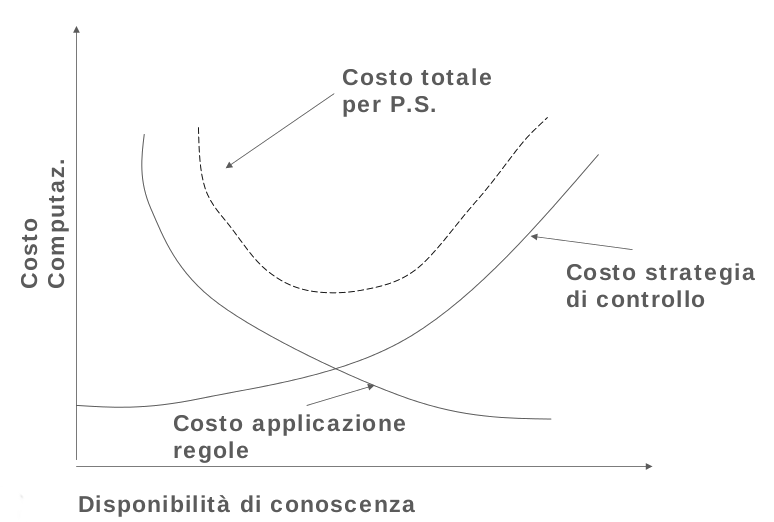
\includegraphics[scale=0.4]{pictures/costprod}
  \caption{Costo di un production system.}
  \label{fig:costo}
\end{figure}


Dall'esempio si evince che, all'aumentare della dimensione degli insiemi di fatti e regole il problema diventa intrattabile utilizzando scansioni lineari per ogni ciclo recognize-act. Inoltre, la funzione \verb!match! specificata esegue ulteriori controlli componente a componente per pattern, per cui si nota come il processo di \emph{matching} non sia banale.\\
Per quel che riguarda la risoluzione dei conflitti, è evidente che, se si definisse un insieme di regole, in cui, per ogni ciclo ne sia applicabile una ed una sola, allora si avrebbe un flusso deterministico paragonabile alla programmazione imperativa. Ciò che invece risulta essere tipico dei sistemi a regole è proprio il non-determinismo. Quest'ultimo è ancor più presente quando i pattern non sono composti solo da costanti ma anche da variabili. Tuttavia, affidarsi al totale non-determinismo è spesso controproducente in termini di efficienza nella ricerca di soluzioni per problemi di una certa consistenza (pur disponendo di un ottimo algoritmo di matching), motivo per cui, oltre alla risoluzione dei conflitti fornita di default da un interprete di regole, è possibile definire strategie di controllo del ragionamento attraverso \emph{meta-regole}, le quali modellano in modo più dettagliato relazioni ed oggetti di dominio. Da ciò si deduce che, una rappresentazione dettagliata e approfondita della conoscenza implica un costo più basso di attivazione delle regole. La figura ~\ref{fig:costo} esplica esaustivamente il concetto \footnotemark. 

\footnotetext{Principles of Artificial Intelligence (Nilsson, 1980).}

Nello sviluppo del sistema TURTLE si è considerato come software di riferimento il tool CLIPS (derivante dalla famiglia \verb!OPS5!)\footnote{C Language Production system - \url{http://clipsrules.sourceforge.net/}.}. Questo software fornisce diversi approcci per la rappresentazione della conoscenza per realizzare un sistema esperto. CLIPS è un sistema \emph{\textbf{forward chaining}} (concatenazione in avanti) in cui il match avviene tra le parti sinistre delle regole e la working memory mentre le azioni sono specificate nelle parti destre. Di conseguenza, anche TURTLE lavora concatenando in avanti. In contrapposizione al \emph{\textbf{backward chaining}}, che ha un approccio \emph{top-down}, il forward chaining è associato ad un approccio \emph{bottom-up}. Sebbene la concatenazione di simboli all'indietro sia indispensabile per problemi top-down (partendo da possibili goal), nulla vieta di risolvere il problema implementando il ragionamento all'indietro tramite forward chaining.

Essendo CLIPS un sistema molto vasto, in questo documento tratteremo solo le caratteristiche da cui si è attinto per realizzare TURTLE. Gli elementi fondamentali di entrambi i sistemi, ed in generale di tutti i sistemi a regole di produzione, sono i \textbf{fatti}, le \textbf{regole} ed il \textbf{meccanismo di matching}.
Per quel che concerne i fatti, la struttura del fatto preso in considerazione è l'\textbf{ordered fact} (fatto ordinato), definito formalmente come una ennupla $(\mu, \sigma_1, ..., \sigma_n)$, dove $\mu$ è il nome del fatto mentre ciascun $\sigma_i$ rappresenta un valore indicizzato per posizione.

\begin{figure}[here]
  \verb!    (padre Mario Gianni)!\\
  \verb!    (padre Antonio Nicola)!\\
  \caption{Una lista di fatti ordinati in CLIPS compatibile con TURTLE. Relazione padre-figlio.}
\end{figure}

\begin{figure}[here]
  \verb!    (defrule <nome-regola>!\\
  \verb!        (condizione_1)!\\
  \verb!        ...!\\
  \verb!        (condizione_m)!\\
  \verb!        =>!\\
  \verb!        (azione_1)!\\
  \verb!        ...!\\
  \verb!        (azione_n)!\\
  \verb!    )!
  \caption{Struttura della definizione di una regola in CLIPS compatibile con TURTLE. Si evince la sintassi LISP-like.}
\end{figure}


\section{I sistemi esperti}

Un sistema esperto è un programma, basato su conoscenza, che tenta di riprodurre il comportamento di un esperto umano in uno specifico dominio. In particolare fornisce le risposte o i consigli che fornirebbe l'esperto umano ed è in grado di giustificare la propria risposta.
I sistemi esperti consentono di risolvere problemi, la cui soluzione richiede una considerevole esperienza umana, ragionando euristicamente su una rappresentazione parziale della realtà del problema.

\begin{figure}[here]
  \centering
  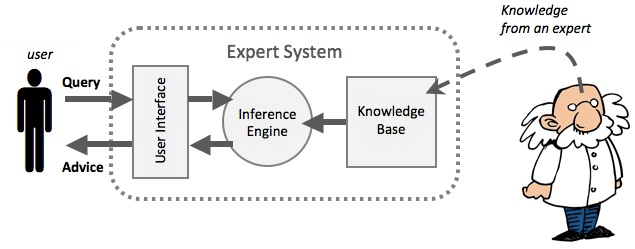
\includegraphics[scale=0.6]{pictures/expertsys}
  \caption{Come funziona un sistema esperto.}
  \label{fig:expertsys}
\end{figure}

Un sistema esperto è costituito da un'interfaccia, che ha il compito di rendere la comunicazione tra utente e sistema più naturale possibile, da una \emph{base di conoscenza}, che memorizza la conoscenza estratta dall'esperto (tale conoscenza consiste, essenzialmente, di fatti e di regole) e da un \emph{motore inferenziale}, parte attiva del sistema, che utilizza la base di conoscenza per inferire nuovi fatti e produrre soluzioni, ovvero simula il processo di ragionamento tramite il quale è possibile trarre delle deduzioni logiche partendo dall'esperienza presente nella base di conoscenza, ampliandola.

Un sistema esperto, inoltre, incapsula un modulo per la spiegazione della soluzione che \emph{\textbf{fornisce indicazioni sulle modalità di ragionamento}} e di \emph{\textbf{giustificazione delle scelte intraprese}} per giungere ad una soluzione.


\chapter{TURTLE}
TURTLE è un tool per lo sviluppo di sistemi basati sulla conoscenza codificata mediante fatti e regole di produzione. Il sistema si ispira a CLIPS per ciò che concerne la sintassi dei programmi accettati, la modalità di interazione con l'utente e cerca di replicare gli aspetti peculiari dell'algoritmo di matching RETE. L'attenzione di questo capitolo è rivolta alla descrizione del parser, della rappresentazione dei fatti e delle regole, ad una descrizione dell'algoritmo di matching, nonché della procedura di risoluzione dei conflitti ed infine, della shell d'interazione.

\section{Il parser}
Il parser è il modulo di TURTLE che si occupa del caricamento e della verifica sintattica di un file di testo contenente i costrutti accettati per la rappresentazione di fatti, regole e variabili globali. La grammatica di riferimento utilizzata è un sottoinsieme della grammatica di CLIPS, la cui versione versione integrale è riportata in forma BNF sul suo manuale di riferimento\footnote{\url{http://clipsrules.sourceforge.net/documentation/v630/bpg.pdf}}.

L'implementazione del parser del sistema sfrutta i servizi offerti dalla libreria \textbf{pyparsing}\footnote{\url{http://pyparsing.wikispaces.com/}}, la quale permette la costruzione di una grammatica BNF estesa mediante la composizione di particolari classi, ciascuna delle quali rappresenta uno specifico costrutto del linguaggio. La classe implementata per il parsing costruisce delle liste di coppie ordinate del tipo \verb!(nome costrutto, AST)!, dove AST è un \emph{Abstract Syntax Tree} tipizzato costituito da liste annidate contenenti i costrutti ed i termini riconosciuti per quel particolare costrutto. È possibile, inoltre, inserire commenti di riga tra un costrutto e l'altro all'interno del file specificando come primo carattere il simbolo \verb!";"!, oppure commentare uno o più costrutti utilizzando le sequenze di simboli \verb!"/*"! e \verb!"*/"! rispettivamente per iniziare e terminare un commento multiriga. Nell'appendice A di questo documento è presente la grammatica BNF estesa implementata dal sistema.

\section{Rappresentazione dei fatti}

La scelta progettuale per la rappresentazione dei fatti è ricaduta sui fatti ordinati, costituiti da un nome e da una sequenza di valori. L'ordine dei valori è determinante ai fini del riconoscimento. Per garantire la futura espandibilità del sistema è stata implementata una interfaccia \emph{Fact} dalla quale deriva la classe specifica \emph{OrderedFact}, che rappresenta un fatto ordinato. Si potrebbero in questo modo supportare i fatti non ordinati in future versioni del sistema. La classe \emph{OrderedFact} comprende il nome del fatto ed una lista di valori associati. La classe \emph{Builder} si occupa della lettura dei fatti ottenuti dal parser e dell'inserimento, previa valutazione di eventuali variabili globali ed espressioni costanti, nella lista dei fatti individuati, i quali verranno interpretati dalla classe \emph{Network} ai fini della fase di \textbf{match} prima dell'inserimento nella \emph{Working Memory}.

La \emph{Working Memory} è stata realizzata utilizzando due dizionari: il primo associa ai fatti un valore booleano, che indica se un fatto con tale nome è già stato inserito, e il secondo indicizza i WME a partire dal loro identificativo numerico univoco, in modo da permetterne un facile ritrovamento ed eliminazione. L'inserimento di un fatto nella \emph{Working Memory} determina la costruzione del WME corrispondente, che verrà restituito dopo tale aggiunta. Non si permette l'inserimento di fatti aventi lo stesso nome. L'ausilio dei due dizionari permette l'inserimento, il ritrovamento e la rimozione dei fatti in un tempo costante.

\section{Rappresentazione delle regole}
Per la rappresentazione delle regole si è deciso di implementare una classe \emph{Rule} costituita dal nome della regola, da una lista contenente la parte sinistra, da una lista contenente la parte destra e da un valore numerico di priorità identificato da \emph{salience}. La classe \emph{Builder} si occupa della lettura delle regole ottenute dal parser e dell'inserimento, previa valutazione di eventuali variabili globali ed espressioni costanti, nella lista delle regole individuate, le quali verranno interpretate dalla classe \emph{Network} ai fini della fase di \textbf{build} prima dell'inserimento nella \emph{Production Memory}.

La \emph{Production Memory} è stata realizzata utilizzando un dizionario indicizzato rispetto al nome della regola. In caso di inserimento di una regola avente lo stesso nome di un'altra regola già presente, si sostituisce tale regola con quella che si intende aggiungere. L'ausilio del dizionario permette il ritrovamento di una regola e la verifica di duplicati in un tempo costante.

\begin{figure}[!ht]
  \centering
  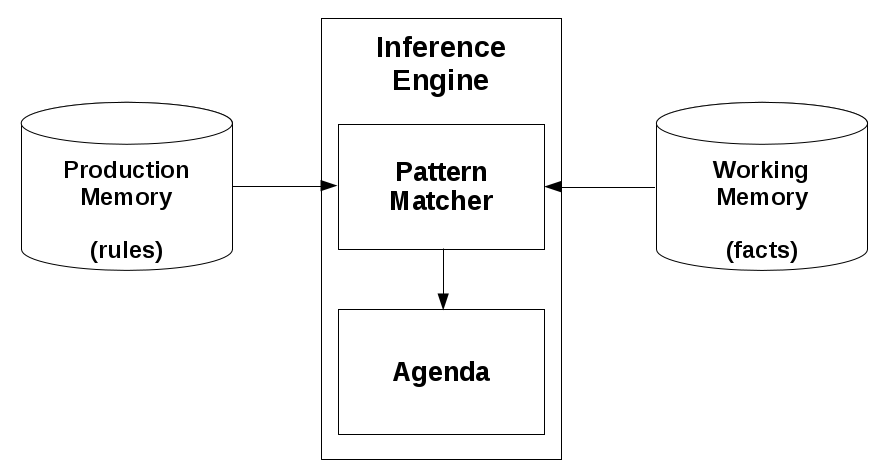
\includegraphics[scale=0.35]{pictures/engine}
  \caption{Architettura di un inference engine.}
\end{figure}


\section{L'algoritmo di matching}
Il modulo di matching del sistema si basa sull'implementazione dell'algoritmo RETE. Per la sua efficienza, rappresenta un punto d'inizio per ricerche, miglioramenti e discussioni nell'ambito dello sviluppo di un motore inferenziale. Il concetto alla base di RETE è quello della scomposizione atomica di tutte le parti sinistre delle regole e della costruzione di un grafo per la verifica di un singolo fatto in una prima fase e successivamente di più fatti congiunti da uno o più predicati.
I punti di forza di questo algoritmo sono:
\begin{itemize}
\item L'\textbf{utilizzo di memorie} (alfa e beta) contenenti riscontri parziali, le quali permettono di ridurre il numero di controlli effettuando un match solo su un nuovo fatto asserito, senza verificare nuovamente i fatti già presenti nella working memory.
\item La \textbf{condivisione dei nodi} tra regole di produzione che hanno stesse condizioni in comune sia nell'alfa network che nella beta. In TURTLE, attualmente, la condivisione dei nodi avviene solamente nell'alfa network; ciò comporta una duplicazione di nodi nella beta network. 
\end{itemize}

RETE presenta anche alcuni svantaggi che naturalmente coinvolgono anche l'algoritmo di matching realizzato per TURTLE:
\begin{itemize}
	\item Si verificano \textbf{sprechi di memoria} dovuti alla duplicazione di riferimenti ai token (nonché ai wme) nelle beta memory.
	\item L'\textbf{eliminazione} di uno o più fatti rappresenta un'operazione non banale all'interno del grafo poiché andrebbero rimossi tutti i riferimenti ed i token generati in cui tali fatti compaiono (operazione denominata retract).
	\item Spesso si verificano \textbf{propagazioni nulle} tra i nodi beta che non avranno mai un'attivazione destra (o solo pochi di essi andranno avanti). Tale problema viene definito ``\emph{utility problem}''\cite{minton1990quantitative}.
		\item Le \textbf{performance} possono diventare drastiche se le condizioni nelle regole sono definite in un ordine sparso, con test ridondanti ed eccessive ritrattazioni.
\end{itemize}

Nella definizione di matching rientra esclusivamente l'algoritmo che viene eseguito quando si verificano attivazioni destre e sinistre. Tuttavia, per permettere tali operazioni e renderle meno costose, esiste una fase di costruzione e definizione delle strutture, pronte per essere attraversate in fase di matching. Per cui, è necessario distinguere la fase di \textbf{build} da quella di \textbf{match}: la prima viene eseguita subito dopo il parsing e l'interpretazione del file, costruendo la rete (alfa e beta), distribuendo i test nei punti opportuni e collegando i pattern di una medesima produzione tra di loro; la seconda, invece, attraversa i suddetti nodi, esegue i test nei nodi che prevedono determinati controlli ed infine costruisce e propaga dei record di fatti denominati \emph{token}.

\subsection{Alfa Network}
La parte alfa della rete è composta da un nodo radice (\textbf{root node}), da nodi alfa (\textbf{alfa node}) e da nodi di memoria (\textbf{alfa memory}).

\subsubsection{Fase di costruzione}
La \textbf{costruzione} dell'\emph{alfa network} avviene in avanti partendo da un nodo radice fino a raggiungere i nodi delle memorie alfa.

Dopo aver costruito un \emph{nodo radice}, si collegano ad esso i \emph{nodi alfa} che rappresentano il nome di ciascun pattern. Ad ogni diramazione corrisponde la scomposizione di un pattern. Se due o più pattern aventi lo stesso nome presentano gli stessi campi a partire dal primo, allora condividono tutti i nodi in comune fino a quanto non presentano campi diversi. I nodi terminali, cioè i nodi foglia, di ciascuna diramazione dell'alfa network sono dei \emph{nodi alfa memory}, nei quali vengono memorizzati i \emph{WME} riconosciuti dalla rete alfa.

L'alfa network è costruita mediante la chiamata di un metodo di \textbf{build}, presente nelle classi che rappresentano i nodi di tale rete. A ciascun nodo è delegata la costruzione del nodo successivo e la chiamata del metodo di build del nodo appena costruito. I nodi rappresentano i propri figli mediante dizionari di nodi indicizzati rispetto all'etichetta che ne rappresenta il campo corrispondente. La scelta del dizionario per la rappresentazione dei figli di un nodo è dettata dalla necessità di dover individuare immediatamente, durante la fase di build, la necessità di condividere o no un nodo e, durante la fase di \textbf{match}, il nodo corrispondente al successivo valore di un fatto. Il modello di riferimento è stato quello della \emph{Data Network with Hashing}\footnote{\url{http://reports-archive.adm.cs.cmu.edu/anon/1995/CMU-CS-95-113.pdf}}.

Il metodo di build del \emph{root node} riceve in input un pattern e costruisce un figlio di tipo \emph{alfa node} o ne condivide uno già esistente, a seconda che il nodo abbia o no un figlio con l'etichetta corrispondente al primo elemento di tale pattern; in seguito tale metodo richiama il metodo di build del nodo appena costruito.

Il metodo di build della classe \emph{alfa node} riceve in input un pattern e un dizionario, inizialmente vuoto, delle variabili incontrate durante la scansione del pattern. Il metodo in questione memorizza nel nodo corrente un valore di profondità, che indica la posizione, incrementata di una unità, del campo del pattern che si sta considerando, in modo da facilitare la successiva fase di match, dato che si stabilisce una corrispondenza uno-ad-uno tra campo del pattern e campo di un fatto. Il valore di profondità è uguale a 0 per il primo campo successivo al nome del pattern, ovvero per il primo livello di nodi alfa costruiti. Il metodo di build dei nodi alfa, in modo analogo a quanto detto per il nodo radice, costruisce un figlio, dato da un altro nodo alfa, o ne condivide uno esistente, a seconda che il nodo abbia o no un figlio con l'etichetta corrispondente al campo che si sta considerando; in seguito si richiama il metodo di build del nodo appena costruito.

La rappresentazione dei nodi alfa prevede, oltre al dizionario di figli indicizzati per campo e al valore che indica la profondità di tali nodi, anche l'etichetta dei nodi in questione, un insieme di riferimenti ai figli che corrispondono per eventuali variabili, fondamentale per evitare l'iterazione su nodi che rappresentano costanti durante il match di variabili, e un riferimento all'ultima variabile, se presente, con il nome analogo all'eventuale nome di variabile del nodo corrente, utile ai fini del controllo di uguaglianza in caso di variabili duplicate in uno stesso pattern.

Nel caso in cui si sia giunti alla costruzione dell'ultimo nodo dell'alfa network per il pattern corrente, allora si costruisce un nodo di tipo alfa memory, collegato al nodo corrente, e si richiama il metodo di build di tale nodo, il quale restituisce un riferimento a se stesso, che verrà propagato lungo le chiamate precedenti, finché non viene restituito a ritroso fino alla chiamata del metodo di build del nodo radice. Ciò permette la memorizzazione del riferimento di ciascuna memoria alfa dell'alfa network, ai fini del collegamento della beta network all'alfa network.

\subsubsection{Fase di matching}
La fase di \textbf{match} dell'\emph{alfa network} è effettuata mediante la chiamata di un metodo di \textbf{match} presente nelle classi che rappresentano i nodi di tale rete. Il metodo di match riceve in input un WME e verifica se, nel dizionario dei figli del nodo corrente, vi è un nodo con etichetta uguale al campo corrente del WME, individuato mediante l'attributo locale di profondità costruito in fase di build: in tal caso si richiama il metodo di match del figlio corrispondente. Se il nodo corrente è stato etichettato come duplicato di una variabile precedente, allora si sfrutta tale riferimento per il controllo dei duplicati. Nel caso in cui l'insieme di riferimenti ad eventuali figli che rappresentano variabili, allora si richiama il metodo di match di tali nodi. Se è stata raggiunta la fine del pattern, e quindi se la fase di match per il WME corrente abbia avuto esito positivo fino al termine dell'alfa network, allora si richiama il metodo di \textbf{attivazione della beta network} presente nella memoria alfa associata al nodo terminale.

Il metodo di attivazione della beta network, presente ne nodi che rappresentano le memorie alfa, prevede la memorizzazione del WME ricevuto in input nella memoria interna del nodo costituita da un dizionario ordinato di WME indicizzate rispetto al loro identificativo numerico (tale struttura dati consente una facile rimozione delle WME durante eventuali operazioni di ritrattazione). Vengono inoltre memorizzate le istanze delle variabili identificate all'interno del pattern che ha superato la fase di match. Si richiama a quel punto il metodo di attivazione del \textbf{match} della \textbf{beta network}.

\subsection{Beta Network}
La parte beta della rete è composta da nodi di join (\textbf{join node} e \textbf{dummy join node}), nodi di memoria (\textbf{beta memory}) e da nodi di tipo production (\textbf{pnode}).

\subsubsection{Fase di costruzione}
La costruzione della \emph{beta network} avviene a ritroso partendo da un \emph{production node} fino a raggiungere i nodi terminali rappresentati dalle memorie della rete alfa già generate.

Partendo da una regola, si scandisce ciascun pattern (test esclusi), si genera un nodo di join associando a quest'ultimo, come input destro, la memoria alfa del pattern; si crea un nodo di memoria beta per l'input sinistro e si ripetono scansione e costruzione sul pattern successivo fino al termine della scansione della parte sinistra di una regola.
L'ultimo pattern letto è associato ad una memoria alfa tramite un nodo dummy join.

Nel caso in cui una regola sia composta esclusivamente da un singolo pattern, viene stabilito un link diretto al \emph{production node}, il quale, nella fattispecie, si occuperà di verificare ciascun WME in arrivo dalla memoria alfa associata ed eventualmente provvederà a far scattare l'attivazione della regola di riferimento. 

Durante la costruzione della rete, se un pattern è nella forma di un \emph{assigned pattern ce}, allora si memorizza nel nodo di join il rifermento alla variabile che conterrà l'istanza di un pattern.

Inoltre, si memorizzano i test che coinvolgono le variabili di ciascun pattern all'interno del nodo di join di competenza: in fase di matching, in seguito al binding delle variabili, verranno eseguiti i test per verificarne il contenuto.

I test e le variabili si possono trovare anche in un production node qualora esista un collegamento diretto ad una memoria alfa.

L'implementazione delle memorie beta è stata realizzata utilizzando dizionari ordinati, i quali permettono un ritrovamento in un tempo ridotto rispetto ad una lista, mantenendo l'ordine di arrivo dei token. Ciò favorisce una riduzione dei tempi in fase di \emph{retract}. Per ciò che concerne le variabili, invece, esse sono memorizzate in dizionari nella forma etichetta-valore.


\subsubsection{Fase di matching}
Quando un WME arriva in una memoria alfa, esso è pronto per essere propagato attraverso la beta network.

Un nodo \emph{beta memory} contiene istanze parziali di regole di produzione, cioè combinazioni di WME che soddisfano in parte una o più regole, cosiddetti \textbf{token}.

Un nodo \emph{join node} ha \emph{due input}: uno \emph{sinistro} a cui è associata una memoria beta ed uno \emph{destro}, a cui è connessa una memoria alfa. Ogni nodo di join si occupa sia di effettuare il binding delle variabili, in comune e non, tra condizioni diverse, che di effettuare i test sugli input ricevuti. L'input sinistro è rappresentato da un token in arrivo dalla memoria beta mentre quello destro è dato da un WME proveniente dalla memoria alfa.

Il binding delle variabili in comune consiste nel verificare che, tutte quelle aventi lo stesso nome, sia nel token che nel WME considerati, abbiano anche lo stesso valore.

Quando un token giunge in un nodo join si parla di \textbf{attivazione sinistra} mentre l'arrivo di un WME fa scattare un'\textbf{attivazione destra}; le attivazioni non possono verificarsi contemporaneamente ed il processo di matching non procede finché non abbiano luogo entrambe: un'attivazione deve attendere il verificarsi dell'altra per poter proseguire la fase di matching.

Se esistono input validi da sinistra e da destra, allora il nodo join si occupa di generare un nuovo elemento unendo i due input in un nuovo token da inviare alla beta memory figlia.
Un caso speciale è rappresentato dal nodo di tipo dummy join che possiede un solo input al quale è associata una memoria alfa (input destro): quando un WME supera il matching nell'alfa network, viene incapsulato in un nuovo token dal dummy join ed il matching prosegue. Il matching in un nodo di join è descritto negli algoritmi \ref{alg:leftactivation} e \ref{alg:rightactivation}.

Le memorie beta ed alfa permettono di riconsiderare rispettivamente token e WME respinti precedentemente, quando certe condizioni sono soddisfatte, con il vantaggio di evitare la ripetizione della fase di matching per ognuno di essi.

Se un token giunge in un \textbf{production node}, allora tutte le condizioni della regola rappresentata dal nodo sono soddisfatte e scatta l'attivazione di quest'ultima; l'insieme delle azioni, presenti nella parte destra della regola, viene aggiunto al conflict set. Il nodo che rappresenta una produzione viene  raggiunto in ultima istanza, per cui rappresenta un nodo terminale. Nelle figure \ref{fig:beta} e \ref{fig:beta1} si possono osservare esempi di matching.

Ogni volta che avviene una propagazione da un nodo di join, vengono generati un nuovo token ed un nuovo dizionario di variabili, unendo le variabili del token considerato con quelle del WME considerato.

\begin{figure}[!ht]
\centering
\begin{verbatim}

		Regole:            Fatti:
		
		    (R1 (f1 ?x)      (fl e1)
		        (f2 ?x)      (f2 e1)
		       ==>....)      (f1 e2)
		                     (f2 e2)
		                     
		Rete:
		             +----------+
		             |   ROOT   |
		             +----------+
		               /      \      		       
		              /        \        
		             /          \        
		        +--------+   +--------+	
		        |   f1   |   |   f2   |   
		        +--------+   +--------+
		            \            /		     
		             \          /
		              \        /
		    x          \      / 
		    =           \    /
		    e1        +--------+ 
		    e2        |  JOIN  |
		              +--------+
		                  | 
		                  |
		                  R1   per x = e1: (f1 e1), (f2 e1)
		                       per x = e2: (f1 e2), (f2 e2)

\end{verbatim}
\caption{Esempio di matching.}
\label{fig:beta1}
\end{figure}

Come già accennato, la fase di ritrattazione di fatti dalla Working Memory implica la cancellazione di tutte le occorrenze dei WME relativi dalla rete, nonché di tutti token in cui tali WME sono presenti. Un token o un WME, quindi, viene eliminato solo quando è eseguita un'azione di \textbf{retract}, altrimenti resta nelle memorie dove occorre, in attesa di partecipare ad un nuovo match.

\begin{algorithm}[h]
 %\SetAlgoLined
 \KwDati{token}
 \KwRisult{new token}
 \Sea{esistono WME nella memoria alfa}{
 	determina le variabili in comune tra le memorie alfa e beta\;
 	\PerCiascun{WME}{
		confronta le istanze delle variabili nel WME rispetto al token\;
		\Sea{il matching va a buon fine}{
			fondi le variabili delle memorie alfa e beta\;
			esegui i test\;
				\Sea{i test sono andati a buon fine}{
					recupera i pattern assignment per il token in input\;
					costruisci un nuovo token Token(token in input, WME corrente)\;
					propaga ai figli del nodo il nuovo token generato, le variabili ed i pattern assignment\;
				}
		}
 	}
 }
 
\caption{Beta network - Attivazione sinistra di un nodo join.}
\label{alg:leftactivation}
\end{algorithm}


\begin{algorithm}[h]
 %\SetAlgoLined
 \KwDati{WME}
 \KwRisult{new token}
 \Sea{esistono token nella memoria beta}{
 	determina le variabili in comune tra le memorie alfa e beta\;
 	\PerCiascun{token}{
		confronta le istanze delle variabili nel token rispetto al WME\;
		\Sea{il matching va a buon fine}{
			fondi le variabili delle memorie alfa e beta\;
			esegui i test\;
				\Sea{i test sono andati a buon fine}{
					recupera i pattern assignment per il token corrente\;
					costruisci un nuovo token Token(token corrente, WME in input)\;
					propaga ai figli del nodo il nuovo token generato, le variabili ed i pattern assignment\;
				}
		}
 	}
 }
 
\caption{Beta network - Attivazione destra di un nodo join.}
\label{alg:rightactivation}
\end{algorithm}

\newpage
\begin{figure}[!ht]
    \vspace*{-2cm}
    \makebox[\linewidth]{
      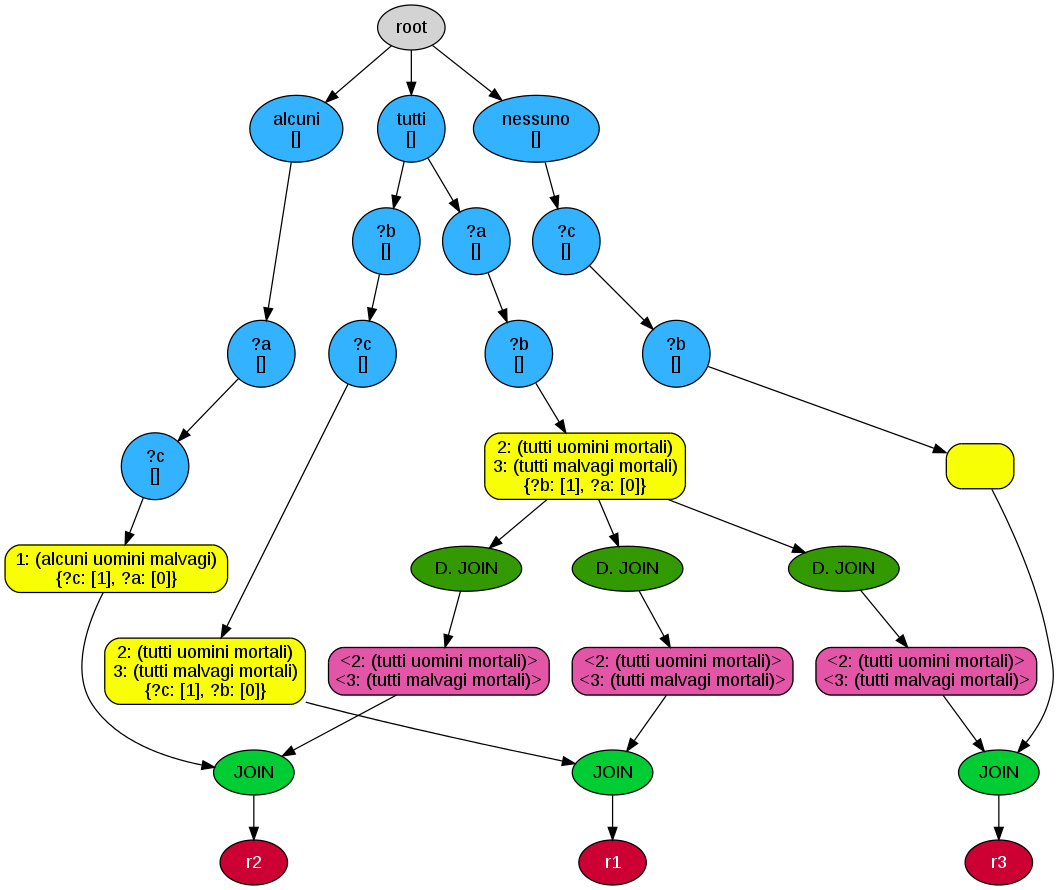
\includegraphics[width=1.4\linewidth]{pictures/beta}
    }
    \caption{Matching beta network per il programma Sillogismi.clp presente nell'appendice di questo documento.}
   \label{fig:beta}
\end{figure}

\newpage
\section{Risoluzione dei conflitti}
Al termine della fase di matching, viene generata un insieme di regole attivabili le cui condizioni sono soddisfatte dai fatti all'interno della Working Memory. Tale insieme prende il nome di \emph{Conflict Set}. Dal momento che il sistema è ispirato a CLIPS, il conflict set prende il nome di \emph{Agenda}. Il fine dell'insieme determinato è quello di risolvere i conflitti tra le regole attivabili selezionandone una ed eseguendone le azioni presenti nella parte destra. La scelta della regola da applicare è effettuata mediante strategie di risoluzione dei conflitti, le quali ordinano le regole applicabili considerandone le proprietà intrinseche e il loro valore di priorità, che prende il nome di \emph{salience}. Dopo l'ordinamento delle regole viene applicata la prima della lista.


L'agenda implementata in TURTLE è composta da un dizionario che associa le salience delle regole attivabili con le liste delle regole aventi tale salience e da un dizionario che associa a ciascun token il numero di regole che esso attiva. L'agenda, inoltre, tiene traccia della strategia scelta e ne permette il cambiamento.


In TURTLE sono state realizzate le seguenti strategie:
\begin{itemize}
\item\textbf{Depth}: È la strategia, come in CLIPS, di \textbf{default}. Tale strategia ordina le regole attivabili in base al loro tempo di attivazione: le regole attivate dal fatto più recente vengono posizionate al di sopra delle regole aventi la stessa salience attivate dai fatti meno recenti. La strategia in questione è denominata depth poiché è una depth-first-search.
\item\textbf{Breadth}: Le regole attivate dal fatto più recente vengono posizionate al di sotto delle regole aventi la stessa salience attivate dai fatti meno recenti. La strategia in questione è denominata breadth poiché è una breadth-first-search, in cui l'ordine delle attivazioni è gestito come se fosse una coda.
\item\textbf{Random}: Le regole attivabili vengono mescolate in un ordine casuale.
\item\textbf{Simplicity}: Tra tutte le regole con la stessa salience, le nuove attivazioni vengono inserite al di sopra di quelle corrispondenti a regole con uguale o maggiore specificità, definita in base ai seguenti criteri di analisi per la loro parte sinistra:
	\begin{itemize}
	\renewcommand{\labelitemii}{$\cdot$}
	\item\textbf{+1} per ciascun pattern.
	\item\textbf{+1} per ciascuna variabile univoca.
	\item\textbf{+1} per ciascuna funzione o predicato.
	\end{itemize}
\item\textbf{Complexity}: Tra tutte le regole con la stessa salience, le nuove attivazioni vengono inserite al di sopra di quelle corrispondenti a regole con uguale o minore specificità.
\item\textbf{LEX}: È una implementazione Naive della strategia LEX di CLIPS. Le regole attivate dai fatti più recenti vengono posizionate al di sopra delle regole aventi la stessa salience attivate dai fatti meno recenti. Rispetto alla strategia depth la priorità di una regola è data da un ordinamento lessicografico dei fatti che la attivano piuttosto che dall'individuazione del fatto più recente.
\item\textbf{MEA}: È una implementazione Naive della strategia MEA di CLIPS. Le regole in cui il primo fatto dei token che le attivano è più recente vengono posizionate al di sopra di quelle in cui il primo fatto dei token che le attivano è meno recente.
\end{itemize}

\newpage
\section{La shell d'interazione}
Per caricare un programma, eseguirlo, ed interagire con esso, è necessario avviare TURTLE da riga di comando\footnote{Sono necessarie alcune dipendenze, specificate in un file di testo nella directory del progetto.}. Il file da passare in input all'interprete Python è \textbf{Turtle.py} (\textbf{python -B Turtle.py})\footnote{Il parametro ``-B'' serve ad evitare la creazione del file .pyc contenente il bytecode; quest'ultimo permette di avviare rapidamente il sistema, ma non offre alcun vantaggio in fase di esecuzione.}.

Dopo aver avviato il sistema, un prompt sarà a disposizione per ricevere i comandi necessari al caricamento e all'esecuzione di un programma a regole, solitamente contenuto in un file di testo con estensione ``.clp''.

\begin{figure}[!ht]
\centering
\begin{verbatim}
                 __
      .,-;-;-,. /'_\  TURTLE Pre-Release
    _/_/_/_|_\_\) /
  '-<_><_><_><_>=/\   An expert system shell inspired by CLIPS syntax
    `/_/====/_/-'\_\  Running on Python 2.7.3 32bit
     ''     ''    ''
    Usage: help to see online help
           <Tab> to show commands
           <Up-arrow>, <Down-arrow> to scroll through the history
           <Ctrl-c> to break a running program
           <Ctrl-d>, quit or exit to leave


TURTLE> 
\end{verbatim}
\caption{Prompt della shell.}
\label{fig:prompt}
\end{figure}

Nella figura \ref{fig:prompt} viene mostrato come si presenta il prompt dei comandi all'avvio del sistema. L'interfaccia testuale propone un banner informativo con le scorciatoie da tastiera ed i comandi utili per interagire, i quali offrono diverse comodità come la possibilità di richiamare comandi già digitati in precedenza, il completamento automatico e l'help online. 

Quest'ultimo fornisce spiegazioni sull'utilizzo di tutti i comandi oltre che le liste di funzioni e predicati disponibili ed utilizzabili all'interno di fatti e regole. E' possibile eseguire un programma impostando un limite d'esecuzione oltre il quale viene fermato il ciclo riconosci-agisci, lasciando in agenda tutte le attivazioni non ancora eseguite.

Per fornire compatibilità sintattica con CLIPS, è possibile racchiudere opzionalmente ogni comando tra parentesi tonde; per cui, ad esempio, il comando \textbf{help} è equivalente al comando \textbf{(help)}.

%\vspace{0.5cm}
%\begin{figure}[!ht]
%  \centering
%  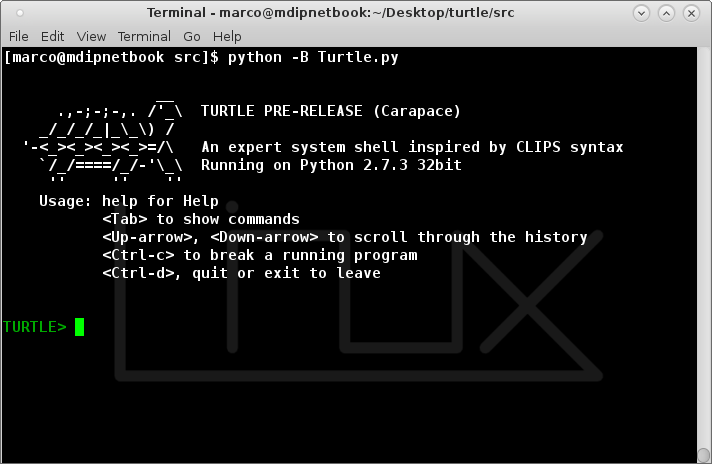
\includegraphics[scale=0.50]{pictures/cmdavvio}
%  \caption{Avvio della shell.}
%  \vspace{0.5cm}
%  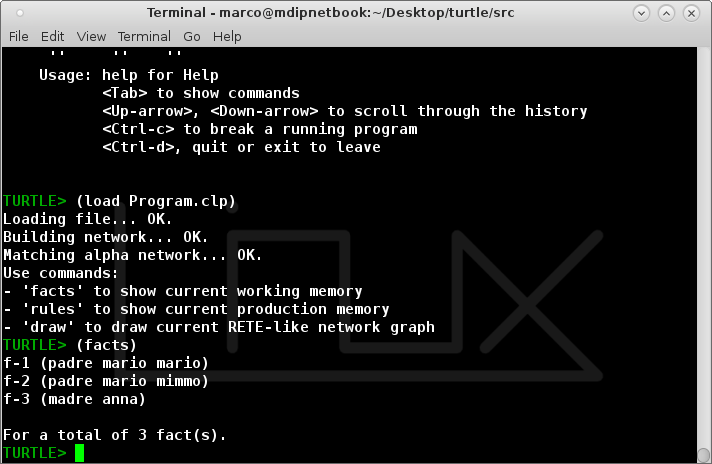
\includegraphics[scale=0.50]{pictures/cmdfacts}
%  \caption{Caricamento di un programma.}
%\end{figure}

La shell dispone del completamento automatico del testo premendo il tasto TAB. Se quest'ultimo viene premuto senza aver digitato alcun carattere, verrà mostrato l'intero elenco dei comandi che è possibile impartire alla shell.

Si possono definire fatti, regole e variabili globali direttamente da shell oltre che caricare uno o più file. Al contrario di CLIPS \footnote{CLIPS, dopo un reset ripristina solo tutti i fatti che sono stati definiti tramite il costrutto deffacts, da shell o da file.}, tutti gli elementi definiti dalla shell tramite \emph{assert} o \emph{deffacts} (oltre quelli caricati da file), dopo un \emph{reset}, saranno mantenuti in memoria. Attualmente la command line non accetta comandi multi-riga.

Se si intende ripulire l'intero ambiente è necessario il comando \emph{clear}, come avviene in CLIPS.

% Capitolo 3

\chapter{Dettagli implementativi}
L'implementazione del sistema è interamente realizzata in \textbf{Python}\footnote{La versione utilizzata è la  2.7.}, un linguaggio di grande supporto all'implementazione immediata di idee, data la sua notevole \textbf{espressività}. Quest'ultima si è rivelata un vantaggio per esprimere e condividere concetti sotto forma di codice chiaro e compatto. Tuttavia, poiché quest'ultimo è interamente interpretato, il problema che si riscontra maggiormente è in alcuni bug che spesso passano inosservati, se non definendo opportuni test grazie al supporto di moduli come il debugger \textbf{pdb} \footnote{E' possibile mandare in esecuzione il sistema in modalità debug utilizzando come parametro aggiuntivo \textbf{-m pdb} (\url{http://docs.python.org/2/library/pdb.html}).}.

\section{Il sistema dei tipi}

I tipi di dati realizzati fanno riferimento a quelli proposti da CLIPS (nonché dal linguaggio LISP). Utilizzando l'ereditarietà, si è definito un tipo di base denominato \textbf{BaseType} dal quale derivano tipi che a loro volta sono superclassi e costituiscono la seguente gerarchia:

\begin{itemize}
	\item \textbf{BooleanType}: rappresenta un valore booleano e si indica con i simboli \verb!TRUE! e \verb!FASLE!.
	\item \textbf{NumberType}: superclasse per la definizione di tipi numerici.
		\begin{itemize}
			\item \textbf{IntegerType}: rappresenta un valore intero, positivo o negativo. Il valore intero massimo specificabile è legato all'implementazione in Python\footnote{Il massimo intero specificabile, per Python v2.x, è definito in \emph{sys.maxint} mentre il minimo equivale a quest'ultimo più uno.}.
			\item \textbf{FloatType} :  rappresenta un valore floating point, positivo o negativo. Il valore intero massimo specificabile è legato all'implementazione in Python \footnote{Per maggiori informazioni consultare \emph{sys.float_info}.}.
		\end{itemize}
	\item \textbf{LexemeType}: superclasse per la definizione di tipi alfanumerici.
		\begin{itemize}
			\item \textbf{SymbolType}: rappresenta il tipo maggiormente utilizzato, composto da caratteri alfanumerici e dai simboli ``\verb!-!'' e ``\verb!_!''.
			\item \textbf{StringType}: rappresenta il tipo di dato stringa racchiusa tra doppi apici ``\verb!"!'' e contenente qualsiasi carattere stampabile. Questo tipo si differenzia dal SymbolType per il numero di caratteri utilizzabili e soprattutto per la capacità di poter utilizzare gli spazi.  
		\end{itemize}
	\item \textbf{VariableType}: superclasse per la definizione dei tipi di variabili. Le variabili trattate non prevedono \textbf{wildcard}.
		\begin{itemize}
			\item \textbf{SinglefieldVariableType}: rappresenta una variabile single field che interessa un singolo campo di un fatto o di un pattern. Essa si dichiara all'interno della parte sinistra di una regola e, se necessario, anche nella parte destra. Alcuni esempi di variabili single field sono: 
\verb!?a!, \verb!?var!, \verb!?a1!, \verb!?var1!.
			%\item \textbf{MultifieldVariableType}
			\item \textbf{GlobalVariableType}: rappresenta una variabile globale. Le variabili globali sono condivise durante tutta l'esecuzione di un programma. Hanno una sintassi differente da quelle locali; alcuni esempi sono: \verb!?*data-nascita*!, \verb!?*x*!, \verb!?*y1*!.
		\end{itemize}
	\item \textbf{FunctionType}: superclasse per la definizione dei tipi di funzioni disponibili.
		\begin{itemize}
			\item \textbf{FunctionCallType}: rappresenta una chiamata ad una funzione o ad un predicato utilizzabili sia nelle due parti delle regole che nella definizione di fatti. E' possibile quindi definire un campo di un fatto come il risultato di una determinata funzione che lavori su numeri, stringhe o valori booleani.
			\item \textbf{SpecialFunctionCallType}: rappresenta una chiamata ad una funzione speciale. Le funzioni speciali permettono di interagire e manipolare lo stato del sistema piuttosto che elaborare solo dati come invece fanno le funzioni. Alcuni esempi sono: \verb!assert!, \verb!retract!, \verb!printout!. Si utilizzano nella RHS di una regola eccetto la funzione speciale \verb!test! che viene utilizzata nella LHS per verificare dei predicati sulle variabili.
		\end{itemize}
	%\item \textbf{ConditionalElementType}
\end{itemize} 


\section{Variabili, funzioni e valutazione}
Come già osservato, il sistema supporta l'utilizzo di variabili di differente tipo. Nella versione attuale del sistema è possibile utilizzare le variabili \emph{globali} e \emph{single field}. Esse possono essere utilizzate sia nei fatti che nelle regole, oltre che nelle funzioni.

Quando un fatto viene definito all'interno del costrutto \textbf{deffacts} è possibile utilizzare esclusivamente variabili globali poiché la shell d'interazione non prevede la possibilità di definire variabili locali da riga di comando. In questo costrutto è possibile utilizzare funzioni e predicati che coinvolgano o meno variabili globali; la valutazione delle variabili, di funzioni e di predicati, avviene prima dell'inserimento dei fatti all'interno della working memory. Se una variabile globale non è stata definita o viene utilizzata in una funzione che non accetta parametri del tipo della variabile, il sistema interrompe l'operazione corrente ed un'eccezione viene sollevata.

Nella definizione di un pattern di un fatto, nella parte sinistra della regola, è possibile specificare variabili locali (single field) e globali. Tali variabili concorreranno al match durante il \emph{recognize-act cycle}; non sono ancora presenti pattern conditional element di tipo not e or. Tuttavia, si consideri che, per le variabili, è possibile definire dei test opportuni (sempre nella LHS di una stessa regola) per verificare uno o più predicati.

Se una regola viene attivata, le sue azioni potrebbero consistere nella stampa su \emph{stdout} di contenuti elaborati, nell'asserzione di nuovi fatti o nella ritrattazione di essi. In tali casi è possibile utilizzare variabili globali e locali\footnote{Il controllo della presenza di una variabile locale nella LHS non viene effettuato in fase di parsing per non introdurre ulteriori controlli. Tale inconsistenza si noterà solo in fase d'esecuzione. Si lascia al buon senso e alla responsabilità dello sviluppatore l'attenzione verso questi effetti collaterali.}, funzioni e predicati.

Per tenere traccia delle variabili globali (o condivise) durante l'esecuzione di un programma, è stato realizzato un \textbf{environment} al quale accedono tutte le componenti interessate e che viene condiviso durante tutto il ciclo di esecuzione di un programma, dal parsing del file fino all'esecuzione dell'ultima regola applicabile.
Perciò, quando si rende necessaria la valutazione di una variabile, viene consultato l'environment per ritrovarne il valore corrente.

La visita e la valutazione di variabili, funzioni e predicati avviene tramite la classe \textbf{evaluator}, che si occupa di visitare ciascun nodo in base al suo tipo e di valutarne il contenuto. L'evaluator si compone di un metodo di default che restituisce il nodo visitato nel caso in cui non sia stato definito un comportamento per quel tipo di nodo, e di metodi definiti per ciascun tipo che si occupano di elaborarne il contenuto ove possibile. Infine, è presente il metodo \emph{evaluate} che cerca di valutare il contenuto del nodo richiamando se stesso nel caso in cui vi siano annidamenti (ad esempio nel caso di nodi che contengono funzioni).

Le funzioni ed i predicati possono essere utilizzati quando si definiscono dei fatti, nei test presenti nella parte sinistra della regola e nella parte destra di quest'ultima.

\begin{figure}
\centering
 \begin{verbatim}
      (deffacts
         (soggetto1 eta 30)
         (soggetto2 eta 20)
         ...)

      (defrule maggiore
         (?s1 eta ?x)
         (?s2 eta ?y)
         (test (> ?x ?y))
         =>
         (assert (?s1 maggiore ?s2))
         (printout ?s1 "è più grande di" ?s2)
         (printout "totale:" (+ ?x ?y)))
 \end{verbatim}
 \caption{Utilizzo di variabili e funzioni in una regola.}
\end{figure}

\section{Strutture dati per il conflict set}

La risoluzione dei conflitti implica l'utilizzo di una strategia che riordini l'insieme in base a determinati criteri. In TURTLE, sono stati adottati diversi \emph{container} dati per adattarsi al tipo di strategia utilizzato ed eseguire attivazioni in un tempo costante.
Per le strategie più complesse è stato definito un tipo di dato \textbf{KeyHeapq} allo scopo di riordinare le attivazioni sfruttando una coda con priorità e specificando, a seconda del caso, la chiave per effettuare tale ordinamento.
I container utilizzati sono:
\begin{itemize}
\item \textbf{Lista} per la strategia \textbf{Depth}: permette l'inserimento e la rimozione di un elemento come se fosse una pila\footnote{In Python una lista si può utilizzare come fosse una pila attraverso i metodi \emph{append} e \emph{pop} rispettivamente per inserire e rimuovere elementi dalla coda in un tempo costante.}
\item \textbf{Deque} per la strategia \textbf{Breadth}.
\item \textbf{Lista} per la strategia \textbf{Random}.
\item \textbf{KeyHeapq} per la strategia \textbf{Simplicity} con chiave la \textbf{complessità} di una regola.
\item \textbf{KeyHeapq} per la strategia \textbf{Complexity} con chiave la \textbf{complessità} negativa di una regola.
\item \textbf{KeyHeapq} per la strategia \textbf{LEX} con chiave gli \textbf{indici dei fatti} che soddisfano una regola.
\item \textbf{KeyHeapq} per la strategia \textbf{MEA} con chiave il primo \textbf{indice di un fatto all'interno di un token} che soddisfa una regola.
\end{itemize}


\section{Confronto con CLIPS}

TURTLE, allo stato attuale, supporta solo un piccolo sottoinsieme di feature ereditate da CLIPS, con qualche variazione sintattica.
Le caratteristiche principali sono:
\begin{itemize}
	\item Supporto dei fatti ordinati (senza template).
	\item Presenza di variabili globali definite attraverso il costrutto \textbf{defglobal} ed utilizzabili nella parte destra di una regola, come parametro di una funzione e come campo nella definizione di un nuovo fatto. Rispetto a CLIPS, si è scelto di poter utilizzare le variabili globali anche nella parte sinistra di una regola.
	\item Utilizzo del costrutto \textbf{deffacts} per asserire uno o più fatti con la possibilità di utilizzare funzioni e variabili globali.
	\item Utilizzo del costrutto \textbf{defrule} per definire una regola\footnote{Una regola è considerata valida solo se ha almeno un pattern nella parte sinistra. Ne consegue che non sono ammesse attivazioni di tipo wildcard.}. 
	\item Utilizzo del costrutto \textbf{declare} in defrule per definire le proprietà di una regola. Attualmente l'unica proprietà supportata è la \textbf{salience}.
	\item Presenza di variabili locali \textbf{single field}.
	\item Possibilità di utilizzare la funzione speciale \textbf{test} nella parte sinistra di una regola per verificare uno o più predicati su una o più variabili locali.
	\item Utilizzo della fuzione speciale \textbf{assert} nella parte destra di una regola per asserire uno o più fatti contenenti costanti, variabili globali e variabili locali già presenti nella parte sinistra.
	\item Utilizzo della funzione speciale \textbf{retract} per eliminare uno o più fatti.
	\item Presenza della funzione speciale \textbf{bind} per modificare una variabile globalmente o localmente a seconda del tipo.
	\item Possibilità di variare il criterio di ordinamento del conflict set (agenda) tramite la funzione speciale \textbf{strategy}, sia tramite shell che in fase d'esecuzione, specificando la strategia da adottare tra le azioni nella parte destra di una regola.
	\item Possibilità di stampare contenuti su standard output tramite la funzione speciale \textbf{printout}.
\end{itemize}

Consultare l'help online presente nella shell\footnote{digitare \textbf{help \emph{nome_comando}} per ottenere maggiori informazioni.} per conoscere meglio tali feature.

\section{Estensibilità}
Durante lo sviluppo del sistema, si è cercato di rendere il codice scalabile per sviluppi futuri. L'intento di realizzare un sistema di base che fosse predisposto alla realizzazione di nuove feature è stato al centro del processo di progettazione.

Tra le estensioni che si potrebbero introdurre in futuro, vi sono due punti cruciali che necessitano una certa elasticità per un facile aggiornamento: l'introduzione di nuovi nodi nell'algoritmo di matching e l'inserimento di nuove funzioni utilizzabili con i tipi di dati presenti.

Nel primo caso si è realizzata una superclasse \emph{Node} che è possibile estendere con le caratteristiche del nodo che si intende implementare, mentre, per il secondo caso è stata realizzata una classe denominata \emph{FunctionMapper}, la quale si occupa di caricare le funzioni disponibili leggendo dei file \emph{.py} presenti all'interno della directory in cui specificare nuove funzioni. Tali file estendono la classe \emph{Module}, definita per permettere all'utente di inserire nuovi file \emph{.py} contenenti nuove funzioni e nuovi predicati definiti in base alle proprie esigenze\footnote{Per comprendere meglio come realizzare nuove funzioni e nuovi predicati, consultare i file \emph{Functions.py} e \emph{Predicates.py}.}.

\chapter{Conclusioni}

Allo stato attuale il sistema non supporta diverse componenti che CLIPS fornisce.
Di seguito vengono proposti alcuni sviluppi possibili per il futuro sia a livello di feature che di modifiche architetturali al fine di ottimizzare il sistema.
E' stato effettuato qualche test per verificare le prestazioni del sistema. Ad esempio, è stato riscontrato, su una stessa macchina, che CLIPS esegue 22000 attivazioni al secondo contro le 800 eseguite da TURTLE; stando ad una valutazione preliminare, TURTLE è risultato essere circa 30-35 volte più lento di CLIPS\footnote{Test effettuati su una macchina con processore Intel P8600 2.4GHz. Va considerato anche l'overhead generato da Python rispetto al linguaggio C (con il quale è stato realizzato CLIPS).}.

\section{Sviluppi futuri}

Per semplificare e rendere più flessibili sintassi e semantica si potrebbero introdurre le variabili \textbf{multifield} ed il supporto alle \textbf{wildcard} (? e \$?).

Due conditional element molto utili per evitare duplicazioni di regole e test sono l'\textbf{OR CE}, il \textbf{NOT CE} ed un'analisi per scomporre gli \textbf{AND CE}\footnote{Come già specificato, da non confondere con i predicati \emph{and}, \emph{or} e \emph{not} utilizzabili nei test.}.

Per ciò che concerne la definizione dei fatti, un metodo che fornirebbe maggiore dettaglio nella formalizzazione è quello dei \textbf{template}; in tal caso si parlerebbe di \emph{unordered facts} poiché i fatti in questione sarebbero indicizzati per attributo.

Attualmente, in TURTLE, la rete costruita può essere aggiornata, dopo la costruzione, aggiungendo nuove regole tramite shell o file. Non è possibile rimuovere regole se non ricostruendo l'intera rete.

Per evitare riscritture di regole potrebbe tornare utile l'utilizzo del costrutto \textbf{if-then-else} per avere, all'interno di una regola, una parte destra più articolata.

Il costrutto \textbf{deffunction} di CLIPS fornirebbe un livello di astrazione migliore. Allo stato attuale, è possibile definire le proprie funzioni solamente in Python.

Infine, per fornire tutti gli elementi della logica proposizionale, dovrebbero essere integrati i quantificatori \textbf{forall} (per ogni) ed \textbf{exists} (esiste).

A livello architetturale, sarebbe possibile velocizzare la fase di retract (e di conseguenza l'intero sistema) attraverso la condivisione di memorie beta imputabili agli stessi gruppi di pattern e relativi test. Inoltre, ottimizzazioni nella fase di scomposizione di una regola apporterebbero migliorie in termini di tempo durante la fase di matching distribuendo maggiore carico di lavoro alla fase di costruzione.

Per permettere lo sviluppo incrementale di un programma a regole, risulterebbe molto utile la possibilità di rimuovere regole ed aggiungerne di nuove senza dover ricostruire interamente la rete; inoltre, introdurre il salvataggio di snapshot dello stato attuale del mondo (fatti e regole, sia di partenza che aggiunte o rimosse in fase di run) renderebbe più agile la ripresa di una computazione dopo una terminazione forzata o involontaria del sistema.

Un'implementazione interessante potrebbe essere l'inserimento dell'algoritmo di ricerca informata \textbf{A*} al fine di poter utilizzare un programma \emph{skeleton} da modellare in base al problema da risolvere, specificando, ad esempio, una funzione euristica, una funzione costo di passo o gli stati del problema.

\section{Ringraziamenti}

La realizzazione di questo sistema è stata possibile grazie ai numerosi individui che hanno contribuito al mondo open-source, rilasciando componenti software che si sono rivelate fondamentali per TURTLE.

Grazie anche a coloro che hanno reso disponibili tesi e pubblicazioni inerenti l'algoritmo RETE, documenti fondamentali senza i quali difficilmente avremmo potuto procedere nello sviluppo di un algoritmo di matching RETE-like. 

Infine, ma non per ultimo, un sentito ringraziamento alla \emph{Professoressa Floriana Esposito} per averci trasmesso tenacia, determinazione, motivazione e per aver suscitato in noi studenti, durante il corso di \emph{Ingegneria della Conoscenza e Sistemi Esperti}, un interesse non indifferente verso questa branca dell'intelligenza artificiale.



% appendici
\begin{appendices}
\chapter{Grammatica del linguaggio}
{\textbf{BNF estesa}}
\begin{grammar}
{\large
<printables> ::=  0 | 1 | 2 | 3 | 4 | 5 | 6 | 7 | 8 | 9 | a | b | c | d | e | f | g | h | i | j | k | l | m | n | o | p | q | r | s | t | u | v | w | x | y | z | A | B | C | D | E | F | G | H | I | J | K | L | M | N | O | P | Q | R | S | T | U | V | W | X | Y | Z | ! | \# | \$ | \% | \& | ( | ) | * | + | , | - | . | / | : | ; | \textless{} | = | \textgreater{} | ? | @ | [ | \textbackslash{} | ] | \^{} | \_{} | \{ | \} | \texttildelow{} | \'{} | \"{}

<nums> ::=  0 | 1 | 2 | 3 | 4 | 5 | 6 | 7 | 8 | 9

<alphas> ::= a | b | c | d | e | f | g | h | i | j | k | l | m | n | o | p | q | r | s | t | u | v | w | x | y | z | A | B | C | D | E | F | G | H | I | J | K | L | M | N | O | P | Q | R | S | T | U | V | W | X | Y | Z

<alphanums> ::= a | b | c | d | e | f | g | h | i | j | k | l | m | n | o | p | q | r | s | t | u | v | w | x | y | z | A | B | C | D | E | F | G | H | I | J | K | L | M | N | O | P | Q | R | S | T | U | V | W | X | Y | Z | 0 | 1 | 2 | 3 | 4 | 5 | 6 | 7 | 8 | 9

<sign> ::= \verb!+! | \verb!-!

<unsigned int> ::= <nums>+

<integer> ::= [<sign>]<unsigned int>

<exponent> ::= \{ '\verb!e!' | '\verb!E!' \}<integer>

<float> ::= <integer>'\verb!.!'<unsigned int>[<exponent>]
 \alt <integer><exponent>
 \alt <integer>'\verb!.!'[<exponent>]
 \alt [<sign>]'\verb!.!'<unsigned int>[<exponent>]

<boolean> ::= \verb!TRUE! | \verb!FALSE!

<string> ::= '\verb!"!' <printables>+ '\verb!"!'

<printout string> ::= <printables>+

<comment> ::= <string>

<symbol> ::= <alphas>\{<alphanums>| '\verb!_!' | '\verb!-!' \}*

<constant> ::= <boolean>
\alt<symbol>
\alt<string>
\alt<float>
\alt<integer>

<deffacts name> ::= <symbol>

<variable symbol> ::= <alphas>+<alphanums>*

<global variable> ::= '\verb!?*!'<vairable symbol>'\verb!*!'

<singlefield variable> ::= '\verb!?!'<vairable symbol>

%<multifield variable> ::= '\$?'<vairable symbol>

<variable> ::= <singlefield variable>
%\alt<multifield variable>
\alt<global variable>

<special function names> ::= '\verb!assert!' | '\verb!retract!' | '\verb!bind!' | '\verb!printout!' | '\verb!strategy!'

<function name> ::= <printables>+\\-\{<special function names> | '(' | ')' \}*

<expression> ::= <costant>
\alt<variable>
\alt<function call>

<function call> ::= '(' <function name><expression>* ')'

<fact field> ::= <global variable>
\alt<constant>
\alt<function call>

<ordered fact pattern> ::= '(' <symbol><fact field>* ')'

<fact pattern> ::= <ordered fact pattern>

<deffacts construct> ::= '(' '\verb!deffacts!' <deffacts name>[<comment>]\\<fact pattern>* ')'

<rule name> ::= <symbol>

<integer expression> ::= <expression>

<rule property> ::= '(' '\verb!salience!' <integer expression> ')'

<declaration> ::= '(' '\verb!declare!' <rule property>  ')'

<rhs term> ::= <constant>
\alt <variable>
\alt <function call>

<lhs term> ::= <constant>
\alt <singlefield variable>

<rhs constraint> ::= <rhs term>

<lhs constraint> ::= <lhs term>

<ordered pattern ce> ::= '(' <symbol><lhs constraint>* ')'

<pattern ce> ::= <ordered pattern ce>

<assigned pattern ce> ::= <singlefield variable> '\verb!<-!' <pattern ce>

<test ce> ::= '(' '\verb!test!' <function call>  ')'

%<and ce> ::= '(' '\verb!and!' <conditional element>+ ')'

%<or ce> ::= '(' '\verb!or!' <conditional element>+ ')'

%<not ce> ::= '(' '\verb!not!' <conditional element> ')'

<conditional element> ::= <boolean>
\alt <test ce>
%\alt<and ce>
%\alt<or ce>
%\alt<not ce>
\alt <pattern ce>
\alt <assigned pattern ce>

<conditional elements> ::= <conditional element>*

<rhs pattern> ::= <ordered rhs pattern>

<rhs patterns> ::= <rhs pattern>+

<rhs function call> ::= '(' '\verb!assert!' <rhs patterns>')'
\alt '(' '\verb!retract!' \{<singlefield variable>|<unsigned int>\}+')'
\alt '(' '\verb!bind!' <variable><expression>')'
\alt '(' '\verb!printout!' \{<prinout string>|<expression>\}+')'
\alt '(' '\verb!strategy! \{\verb!depth!|\verb!breadth!|\verb!random!|\verb!complexity!|\verb!simplicity!|\verb!lex!|\verb!mea!\}')'


<action> ::= <rhs function call>

<defrule construct> ::= '(' '\verb!defrule!' <rulename>[<comment>][<declaration>]\\<conditional elements> '\verb!=>!' <action>* ')'

<global assignment> ::= <global variable> '\verb!=!' <expression>

<defglobal construct> ::= '(' '\verb!defglobal!' <global assignment>* ')'

<construct> ::= <deffacts construct>\alt<defrule construct>\alt<defglobal construct>

<line comment> ::= \{'\verb!;!'\}+ <any character until EOL>

<multiline comment> ::= \{'\verb!/*!'\}+ <any character>  + \{'\verb!*/!'\}

<program> ::= \{<construct>|<line comment>|<multiline comment>\}*
}
\end{grammar}



\chapter{Funzioni e Predicati}
\section{Funzioni}

\subsection{NumberType}

Ciascun termine delle seguenti funzioni deve essere numerico (\verb!IntegerType! o \verb!FloatType!) oppure una variabile di tipo numerico che verrà sostituita automaticamente se istanziata correttamente.

\subsubsection{Addition}
\emph{Sintassi}: ($+$ $\mathrm{x_1 \ x_2 \ ... \ x_n}$)\\

Somma i termini $x_1, ..., x_n$. Il passo base è \verb!IntgerType(0)!.


\subsubsection{Subtraction}
\emph{Sintassi}: ($-$ $\mathrm{x_1 \ x_2 \ ... \ x_n}$)\\

Sottrae i termini $x_1, ..., x_n$. Il passo base è $x_n$.


\subsubsection{Multiplication}
\emph{Sintassi}: ($*$ $ \mathrm{x_1 \ x_2 \ ... \ x_n}$)\\

Moltiplica i termini $x_1, ..., x_n$. Il passo base è \verb!IntegerType(1)!.


\subsubsection{Division}
\emph{Sintassi}: ($/$ $ \mathrm{x_1 \ x_2 \ ... \ x_n}$)\\

Divide i termini $x_1, ..., x_n$. Il passo base è $x_1$.


\subsubsection{Module}
\emph{Sintassi}: ($\%$ $ \mathrm{x_1 \ x_2 \ ... \ x_n}$)\\

Calcola il resto della divisione tra i termini $x_1, ..., x_n$. Il passo base è $x_1$.


\subsubsection{Power}
\emph{Sintassi}: ($**$ $ \mathrm{x_1 \ x_2 \ ... \ x_n}$)\\

Calcola la potenza di $x_1$ con esponente il prodotto dei termini $x_2, ..., x_n$. Il passo base è $x_1$.


\subsubsection{Abs}
\emph{Sintassi}: ($abs$ $ \mathrm{x}$)\\

Calcola il valore assoluto di $x$. E' un wrapper per la funzione \verb!abs! di Python.


\subsubsection{Minimum}
\emph{Sintassi}: ($min$ $ \mathrm{x_1 \ x_2 \ ... \ x_n}$)\\

Trova il minimo tra i termini $x_1, ..., x_n$. E' un wrapper per la \verb!min! di Python.


\subsubsection{Maximum}
\emph{Sintassi}: ($max$ $ \mathrm{x_1 \ x_2 \ ... \ x_n}$)\\

Trova il massimo tra i termini $x_1, ..., x_n$. E' un wrapper per la funzione \verb!max! di Python.

\subsubsection{Randint}
\emph{Sintassi}: ($randint$ $ \mathrm{x_1 \ x_2}$)\\

Restituisce un numero intero casuale compreso tra $x_1$ e $x_2$ inclusi. Il primo termine non deve essere necessariamente più piccolo del secondo.

\subsection{LexemeType: StringType}

\subsubsection{Strcat}
\emph{Sintassi}: ($strcat$ $ \mathrm{x_1 \ x_2 \ ... \ x_n}$)\\

Concatena le stringhe $x_1, ..., x_n$ restituendo un nuovo  \verb!StringType!.

\subsubsection{Substr}
\emph{Sintassi}: ($substr$ $ \mathrm{string \ start \ end}$)\\

Restituisce una sottostringa compresa tra gli indici di posizione start ed end (escluso) di una stringa passata in input. La funzione si comporta come lo \emph{slicing} di Python, in cui l'intervallo considerato inizia dalla posizione start e termina nella posizione end-1. Se entrambi gli indici superano il massimo range specificabile, viene restituita l'intera stringa in input. Se uno solo degli indici supera il range di posizioni possibili si hanno due casi: se \verb!start! è out of range allora viene restituita una sottostringa data dagli indici \verb!0! ed \verb!end! (\verb![0:end]!); se \verb!end! è  out of range viene restituita una sottostringa data dagli indici \verb!start! e \verb!ultima posizione stringa in input! (\verb![start:]!).

\subsubsection{Strlen}
\emph{Sintassi}: ($strlen$ $ \mathrm{string}$)\\

Calcola la lunghezza della stringa in input ed utilizza un \verb!IntegerType! come valore di ritorno.

\subsubsection{Strindex}
\emph{Sintassi}: ($strindex$ $ \mathrm{string \ substring}$)\\

Cerca un carattere o una sottostringa all'interno di una stringa e, in caso di successo, restituisce la posizione iniziale della sequenza di caratteri ricercata. In caso contrario viene restituito l'intero negativo \verb!-1!. Il risultato viene memorizzato in un \verb!IntegerType! utilizzato come valore di ritorno.

\subsection{LexemeType: SymbolType}

\subsubsection{Symcat}
\emph{Sintassi}: ($symcat$ $ \mathrm{x_1 \ x_2 \ ... \ x_n}$)\\

Concatena i simboli $x_1, ..., x_n$ restituendo un nuovo  \verb!SymbolType!.


\section{Predicati}

\subsection{NumberType e LexemeType}

Ciascun termine dei seguenti predicati deve essere numerico (\verb!IntegerType! o \verb!FloatType!), una lexeme (\verb!StringType! o \verb!SymbolType!), \verb!BooleanType! oppure una variabile di tipo compatibile che verrà sostituita automaticamente se istanziata correttamente.

\subsubsection{Equal}
\emph{Sintassi}: ($eq$  $\mathrm{x_1 \ x_2 \ ... \ x_n}$)\\

Confronta i termini $x_1, ..., x_n$. Restituisce il valore \verb!TRUE! se i termini sono tutti uguali, altrimenti \verb!FALSE!.


\subsubsection{Not equal}
\emph{Sintassi}: ($neq$  $\mathrm{x_1 \ x_2 \ ... \ x_n}$)\\

Confronta i termini $x_1, ..., x_n$. Restituisce il valore \verb!TRUE! se almeno uno dei termini è diverso dagli altri, altrimenti \verb!FALSE!.

\subsection{NumberType e StringType}

Ciascun termine dei seguenti predicati deve essere numerico (\verb!IntegerType! o \verb!FloatType!), una stringa (\verb!StringType!), \verb!BooleanType! oppure una variabile di tipo compatibile che verrà sostituita automaticamente se istanziata correttamente. Eccezioni sono i predicati logici \verb!and!, \verb!or! e \verb!not! che accettano come parametri esclusivamente dei valori booleani e/o altri predicati.

\subsubsection{Equal}
\emph{Sintassi}: ($eq$  $\mathrm{x_1 \ x_2 \ ... \ x_n}$)\\

Confronta i termini $x_1, ..., x_n$. Restituisce il valore \verb!TRUE! se i termini sono tutti uguali, altrimenti \verb!FALSE!.


\subsubsection{Not equal}
\emph{Sintassi}: ($neq$  $\mathrm{x_1 \ x_2 \ ... \ x_n}$)\\

Confronta i termini $x_1, ..., x_n$. Restituisce il valore \verb!TRUE! se almeno uno dei termini è diverso dagli altri, altrimenti \verb!FALSE!.


\subsubsection{Less than}
\emph{Sintassi}: ($<$  $\mathrm{x_1 \ x_2 \ ... \ x_n}$)\\

Verifica l'esistenza di una relazione d'ordine stretto \verb!<! tra  i termini $x_1, ..., x_n$. Restituisce il valore \verb!TRUE! se i termini sono in ordine crescente, altrimenti \verb!FALSE!.


\subsubsection{Less or equal}
\emph{Sintassi}: ($<=$  $\mathrm{x_1 \ x_2 \ ... \ x_n}$)\\

Verifica l'esistenza di una relazione d'ordine \verb!<=! tra i termini $x_1, ..., x_n$. Restituisce il valore \verb!TRUE! se i termini sono in ordine crescente, altrimenti \verb!FALSE!.


\subsubsection{Greater than}
\emph{Sintassi}: ($>$  $\mathrm{x_1 \ x_2 \ ... \ x_n}$)\\

Verifica l'esistenza di una relazione d'ordine stretto \verb!>! tra i termini $x_1, ..., x_n$. Restituisce il valore \verb!TRUE! se i termini sono in ordine decrescente, altrimenti \verb!FALSE!.


\subsubsection{Greater or equal}
\emph{Sintassi}: ($>=$  $\mathrm{x_1 \ x_2 \ ... \ x_n}$)\\

Verifica l'esistenza di una relazione d'ordine \verb!>=! tra i termini $x_1, ..., x_n$. Restituisce il valore \verb!TRUE! se i termini sono in ordine decrescente, altrimenti \verb!FALSE!.

\subsubsection{Logical and} 
\emph{Sintassi}: ($and$ $\mathrm{x_1 \ x_2 \ ... \ x_n}$)\\

Esegue un \verb!and! logico tra i termini $x_1, ..., x_n$\footnote{I predicati \emph{and}, \emph{or} e \emph{not} sono differenti dai predicati \emph{and ce}, \emph{or ce} e \emph{not ce}. Mentre i primi lavorano sui suddetti predicati, questi ultimi riguardano esclusivamente i \emph{pattern ce} per verificare in fase di matching condizioni di esistenza di fatti nella working memory.}. Restituisce il valore \verb!TRUE! se ogni termine ha un valore \verb!TRUE!, altrimenti \verb!FALSE!. I termini, di solito, sono altri predicati.


\subsubsection{Logical or}
\emph{Sintassi}: ($or$ $\mathrm{x_1 \ x_2 \ ... \ x_n}$)\\

Esegue un \verb!or! logico tra i termini $x_1, ..., x_n$. Restituisce il valore \verb!FALSE! se ogni termine ha un valore \verb!FALSE!, altrimenti \verb!TRUE!. I termini, di solito, sono altri predicati.


\subsubsection{Logical not}
\emph{Sintassi}: ($not$ $\mathrm{x}$)\\

Predicato unario che nega il termine $x$. Restituisce il valore \verb!TRUE! se il termine è \verb!FALSE!, altrimenti \verb!FALSE!. Il termine, di solito, è un altro predicato.

\subsection{Predicati Conditional Element}

Sono predicati utilizzati nella parte sinistra di una regola per verificare una serie di condizioni.

\subsubsection{Test}
\emph{Sintassi}: ($test$ $\mathrm{x}$)\\

Predicato unario che testa una condizione $x$. Restituisce il valore \verb!TRUE! se la condizione verificata è vera, altrimenti \verb!FALSE!. E' utilizzato come wrapper di predicati su costanti e variabili nella \verb!LHS! di una regola ed è un conditional element.




\chapter{Esempi}
% Inserire programmi d'esempio come la rappresentazione di una famiglia


\subsubsection{Sillogismi}

\lstinputlisting[style=customlisp]{examples/Sillogismi.clp}

\vspace{1cm}
\subsubsection{Il problema dei missionari e dei cannibali}

\lstinputlisting[style=customlisp]{examples/MissionariCannibali.clp}

\vspace{1cm}
\subsubsection{Relazioni di parentela}

\lstinputlisting[style=customlisp]{examples/Parentele.clp}

\vspace{1cm}
\subsubsection{Interazioni in una rete sociale}

\lstinputlisting[style=customlisp]{examples/Social.clp}

\vspace{1cm}
\subsubsection{Il mondo dei blocchi (con piano senza limitazioni)}

\lstinputlisting[style=customlisp]{examples/Blocchi.clp}

\vspace{1cm}
\subsubsection{Il gioco dell'otto senza euristica}

\lstinputlisting[style=customlisp]{examples/GiocoOtto.clp}

\chapter{Note di installazione}
%  Dipendenze software

E' obbligatoria l'installazione del pacchetto \verb!pyparsing! versione 1.5.7.

Per sfruttare interamente TURTLE, sono necessari pacchetti aggiuntivi, installabili tramite i tool \verb!pip! o \verb!easy_install!:

\begin{itemize}
\item \verb!colorama! 
\item \verb!termcolor!
\item \verb!networkx!
\item \verb!pydot!
\end{itemize}

E' necessaria, inoltre, l'installazione del tool Graphviz per visualizzare graficamente la rete.

\subsection*{Microsoft Windows\textregistered}

Per installare le dipendenze è consigliabile l'installazione di setuptools eseguendo con python il file al seguente link: \url{https://bitbucket.org/pypa/setuptools/raw/bootstrap/ez_setup.py}.

Al termine dell'installazione sarà possibile utilizzare il tool \verb!easy_install! per poter aggiungere i pacchetti richiesti da TURTLE.

Graphviz è disponibile all'indirizzo \url{http://graphviz.org/Download_windows.php}.


\subsection*{GNU/Linux e Unix\textregistered}

Di solito è già presente il tool \verb!pip! per installare i pacchetti aggiuntivi. In caso contrario, è possibile effettuare l'installazione di \verb!pip! o \verb!easy_install! utilizzando il package manager del sistema.

Graphviz è disponibile per il download diretto all'indirizzo \url{http://graphviz.org/Download..php} oppure l'installazione può essere effettuata attraverso il package manager del sistema.

\end{appendices}

% bibliografia
\cleardoublepage
\phantomsection
\addcontentsline{toc}{chapter}{Bibliografia}
\nocite{*}
\bibliographystyle{alpha}
\bibliography{contents/bibliografia}

\begin{flushright}
\vspace{2cm}
Made with \LaTeX{}
\end{flushright}

\end{document}
